%%%%%%%%%%%%%%%%%%%%%%%%%%%%%%%%%%%%%%START PREAMBLE THAT IS THE SAME FOR ALL EXAMPLES
\documentclass{article}

%Required: You must have these
\usepackage{Sweave}
\usepackage{graphicx}
\usepackage{tabularx}
\usepackage{hyperref}
\usepackage{natbib}
\usepackage{pdflscape}
\usepackage{array}
\usepackage{authblk}
\usepackage{gensymb}

%\usepackage[backend=bibtex]{biblatex}
%you'll want these for pretty captioning
\usepackage[small]{caption}

\setkeys{Gin}{width=0.8\textwidth} %make the figs 50 perc textwidth
\setlength{\captionmargin}{30pt}
\setlength{\abovecaptionskip}{10pt}
\setlength{\belowcaptionskip}{10pt}
% manual for caption http://www.dd.chalmers.se/latex/Docs/PDF/caption.pdf

%Optional: I like to muck with my margins and spacing in ways that LaTeX frowns on
%Here's how to do that
 \topmargin -1.5cm 
 \oddsidemargin -0.04cm 
 \evensidemargin -0.04cm % same as oddsidemargin but for left-hand pages
 \textwidth 16.59cm
 \textheight 21.94cm 
 %\pagestyle{empty} % Uncomment if don't want page numbers
 \parskip 7.2pt  % sets spacing between paragraphs
 %\renewcommand{\baselinestretch}{1.5} 	% Uncomment for 1.5 spacing between lines
\parindent 0pt% sets leading space for paragraphs
\usepackage{setspace}

%cross referencing:
\usepackage{xr}
\externaldocument{/Users/aileneettinger/Documents/GitHub/ospree/docs/budburst/budburst_supp}

%\usepackage{zref-xr}
%\zxrsetup{toltxlabel=true, tozreflabel=false}
%\zexternaldocument*{budburst_supp}

%\doublespacing

%Optional: I like fancy headers
%\usepackage{fancyhdr}
%\pagestyle{fancy}
%\fancyhead[LO]{How do climate change experiments actually change climate}
%\fancyhead[RO]{2016}
 
%%%%%%%%%%%%%%%%%%%%%%%%%%%%%%%%%%%%%%END PREAMBLE 

%Start of the document
\begin{document}

%\SweaveOpts{concordance=TRUE}
\bibliographystyle{..//..//refs/bibstyles/amnat.bst}% 

\title{Chilling dominates spring phenological responses to warming} 
%or Winter temperatures dominate spring phenological responses to warming

\author[1,a]{A.K. Ettinger}

\author[2]{C. Chamberlain}

\author[2,3]{I. Morales-Castilla}

\author[1,2]{D. Buonaiuto}

\author[2,4]{D. F. B. Flynn}

\author[2,5]{T. Savas}
\author[2,6]{J. Samaha}

\author[1,2,6]{E. M. Wolkovich}


\affil[1]{Arnold Arboretum of Harvard University, Boston, Massachusetts 02131, USA}

%\affil[2]{Northwest Fisheries Science Center, National Oceanographic and Atmospheric Association, Seattle, Washington USA}

\affil[2]{Department of Organismic and Evolutionary Biology, Harvard University, Cambridge, Massachusetts, USA}

\affil[3]{Department of Life Sciences, University of Alcal\`a CTRA N-II, KM., 33,600, 28802, Alcal\`a de Henares, Spain}

\affil[4]{U.S. DOT Volpe National Transportation Systems Center, Cambridge, Massachusetts, USA}

\affil[5]{Media Lab Open Agriculture Initiative, Massachusetts Institute of Technology, Cambridge, Massachusetts, USA}

\affil[6]{Forest \& Conservation Sciences, Faculty of Forestry, University of British Columbia, Vancouver, British Columbia, Canada}


\affil[a]{Corresponding author; email: ailene.ettinger@noaa.gov; phone: 781-296-4821; mailing address: 2725 Montlake Blvd. E, Seattle, Washington 98112 USA }

%\date{\today} 
\maketitle %put the fancy title on
%\tableofcontents %add a table of contents
%\clearpage
%%%%%%%%%%%%%%%%%%%%%%%%%%%%%%%%%%%%%%%%%%%%%%%%%%%

% To do:
% Word count is ???, need to cut to 1500-1800 if possible (once happy).

% SciMag: https://www.sciencemag.org/authors/science-information-authors
%https://www.sciencemag.org/authors/instructions-preparing-initial-manuscript
% Only 30 REFS!! (We need to be more careful I think.)
% Reports (up to ~2500 words including references, notes and captions?corresponds to ~3 printed pages in the journal) present important new research results of broad significance. Reports should include an abstract, an introductory paragraph, up to four figures or tables, and about 30 references.
%Science Manuscripts should be assembled in the following order:
% Title: 96 character maximum for Research Articles and Reports
%One Sentence Summary: capturing the most important point should be submitted for Research Articles, Reports and Reviews. These should be a maximum of 125 characters and should complement rather than repeat the title
%Authors:and their affiliated institutions, linked by superscript numbers, should be listed beneath the title on the opening page of the manuscript.
%Affiliations:
%Abstract:
%Main Text:
%References and Notes
%Acknowledgements:

%%%%%%%%%%%%%%%%%%%%%%%%%%%%%%%%%%%%%%%%%%%%%%%%%%%



% In Europe, recent work from many of the most well-studied tree species shows declining responses to temperature, suggesting that the long-term trend towards ever-earlier springs may be stalling \citep{fu2015}.

\par Fundamental research in phenology outlines how three major environmental cues, chilling (cool temperatures, generally occurring in the fall and late winter), forcing (warm temperatures, generally occurring in the late winter and early spring), and photoperiod (daylength), provide multiple routes to budburst each spring, depending on the environment \citep{chuine2016}. For example, in some species a cool winter will lower the amount of forcing required to trigger budburst, compared to a warmer winter \citep{harrington2015}. Additionally, photoperiod may trigger budburst, given low chilling and/or forcing \citep{Basler:2014aa, Caffarra:2011b, zohner2016}. Research suggests that all three cues may underlie spring phenology for many temperate woody species \citep{flynn2018,Basler:2014aa,Caffarra:2011qf}, which could have critical forecasting implications---predicting delays in spring phenology as increased warming reduces chilling in some areas \citep{fraga2019} or where earlier budburst shortens the experienced photoperiod. However, there is strong debate, with some research suggesting some cues---such as photoperiod---may be effectively absent in some species, but dominate in others \citep{zohner2016,koerner2010a}. 

\par Resolving this debate requires overcoming major hurdles to estimate responses to each cue. Studies attempting to estimate cues using long-term observational data \citep[e.g.,][]{vitasse2013, zohner2016} generally fail to overcome the fundamental challenge that all three cues are strongly correlated in nature (e.g., during the transition from winter to spring at temperate latitudes, forcing and photoperiod usually increase in step). In contrast to observational studies, controlled environment experiments can breakdown correlations between the cues. These experiments---most often conducted in growth chambers or similar systems to control temperature and light---have been conducted for decades. They have produced contrasting results, however, potentially due to differences in focal species or study cites \citep{zohner2016,Laube:2014a,Basler:2012,Caffarra:2011b,Caffarra:2011a}. Resolving these discrepancies is critical to accurate predictions of spring phenology, especially as continued warming pushes climate into environmental regimes far beyond historical bounds. 
% IM-C: should we mention one-two examples of such contrasting results? [No space currently ... ]
%JD: here, link with why we need to make good predictions - not just resolving a debate, but addressing a fundamental challenge in global change biology 

% Some studies report that photoperiod is likely to constrain species responses to climatic warming \citep{Basler:2012, Caffarra:2011b,Caffarra:2011a}, whereas others state that photoperiod is not a strong cue \citep{zohner2016,Laube:2014a} and that chilling is more important to current and future trends. 
% Given the declining response to temperature observed in long-term observational studies \citep{fu2015}, a number of studies have tried to tease out evidence that chilling or photoperiod cues are playing an increasingly important role in recent years \citep{Basler:2014aa,zohner2016, Laube:2014a}. This work must overcome the fundamental challenge that all three cues are strongly correlated in nature: e.g., during the transition from winter to spring at temperate latitudes, air temperatures increase (i.e., forcing increases) at the same time that photoperiod increases. 

% We should ONLY report the data that went into the budburst analysis. 
\par Here, we leverage nearly 40 years of controlled environment studies to understand how chilling, forcing, and photoperiod determine budburst timing in woody species. %Using a meta-analytic approach we can synthesize experimental results across many taxa to find generalizable patterns. 
We reviewed 201 papers from controlled environment studies, then extracted data from all experiments that reported budburst responses, yielding data from 72 studies across 39 years and 203 species (Fig. \ref{fig:map}, Table \ref{tab:sp}).%(Table S1, Fig. S1) 
The resulting Observed Spring Phenology Responses in Experimental Environments (OSPREE) database includes only studies for which we could identify forcing, photoperiod, and chilling treatments quantitatively and includes a mix of studies where plant tissue was grown in greenhouses or brought in from the field and exposed to experimental conditions. As chilling was rarely reported, we calculated chilling when possible, using a common but approximate method \citep{richardson1974}, in which chilling does not accumulate below 1.4 \degree C or at high temperatures (see Supplemental Methods). We estimated the effects of chilling, forcing, and photoperiod using a Bayesian hierarchical model. Our model averages over interactions between predictors to estimate both species-level responses (generally yielding more accurate estimates for well-studied species, such as \emph{Fagus sylvatica} and \emph{Betula pendula}), and the distribution from which they are drawn, yielding an estimate of the overall response across species (see Supplemental Materials).

\par Across studies, all cues---chilling, forcing, and photoperiod---advance budburst phenology (Fig. \ref{fig:mu}, Tables \ref{tab:modsz}, \ref{tab:modsnonz}). Chilling was the strongest cue (-2.84 days/standard unit or -8.89 days per chill unit), followed by forcing (-0.79 days/standard unit or -4.36 days per \degree C of warming), and photoperiod (-0.54 days/standard unit or -3.15 days per hour of daylength; Fig. \ref{fig:apc},\ref{fig:fig:2dfieldchillutah},\ref{fig:3dexpchillutah}; Tables \ref{tab:modsz},\ref{tab:modsnonz}; see Supplemental Materials for more details). While photoperiod had the smallest effect among the three cues, our results contrast with the extensive literature suggesting photoperiod is an unimportant cue for many species \citep{zohner2016,koerner2010a}---instead we found it was surprisingly large, even when accounting for its interaction with latitude (see also Supplemental Materials for details, especially Fig. \ref{fig:lat}, \ref{fig:fagsyllat}, Table \ref{tab:lat}). It was also generally consistent across species, only deviating in \emph{Fagus sylvatica}, a species well-known for having a large response to photoperiod (which we also found, Fig. \ref{fig:mu}, \ref{fig:lat}). Species responses to chilling were slightly more variable (variance = 2.07 days per chill unit in the standardized model, Fig. \ref{fig:mu}) than responses to forcing (variance = 0.91 days per forcing unit in the standardized model Fig. \ref{fig:mu}).
\par As temperature is fundamentally altered by climate change, our finding that different ends of the temperature spectrum---chilling and forcing---have the strongest effects on budburst suggests that understanding these cues will be critical for forecasting phenology with climate change. Many previous studies attribute advances in budburst to increased forcing \citep{Basler:2014aa,bradley1999,menzel2006,harrington2015}.
Our results, however, suggest chilling has a greater effect on budburst than forcing (Fig. \ref{fig:mu}, \ref{fig:weinberger}, \ref{fig:lat}; Tables \ref{tab:modsz}-\ref{tab:lat}). This has not been widely suggested previously, perhaps because little work has directly manipulated chilling, and the few studies that have were designed to compare chilling versus photoperiod effects \citep[e.g., ][]{Basler:2014aa,Caffarra:2011qf,Laube:2014a,zohner2016}, not forcing versus chilling effects. 
% Should we add comparisons of chilling and forcing cues? Lizzie found 9 studies that manipulate chilling and forcing- look at these papers

\par A simple interpretation of our results supports the hypotheses that chilling and photoperiod cues may underlie declining sensitivities to warming in long-term Central European data \citep{Rutishauser:2008,yu2010,fu2015}. Under these hypotheses, warming increases forcing and thus advances budburst, but such advances become muted if warming also causes declines in chilling and shorter photoperiods experienced near the timing of budburst 
\citep{koerner2010a}.
This basic agreement between our results and long-term observational trends integrates across experimental conditions that encompass more extreme scenarios than may be seen in nature (Fig. \ref{fig:apc}). A more robust comparison requires examining predictions under conditions closer to those found in nature.
%Assessing the implications of these contrasting cues for future phenological shifts requires examining predictions understanding non-experimental conditions.

% Experimental conditions likely differ from those \emph{in situ}, however; for example, photoperiods in experimental treatments ranged from 8 hours to 16 hours, whereas photoperiods during the spring budburst period (e.g., 1 March through 1 May) range from 11 to 14 hours at latitude 45 \degree. We therefore wanted to put the OSPREE experimental data and model estimates in the context of forecasted and observed environmental conditions. 

\par Reinterpreting our model using climate and phenology data that have led to observations of declining temperature sensitivities in Central Europe suggests that chilling and photoperiod are unlikely to cause the observed declines in sensitivity. Our model predicts such declines only at extreme warming for most sites (see Supplemental Materials). In contrast to the common hypothesis that plants experience less chilling with global warming, we found that---for many sites---total estimated chilling increased with warming (Fig. \ref{fig:fore} A,D), though this varied with local climate prior to warming (Fig. \ref{fig:foremap} - \ref{fig:chillfore}). 
Portions of Central Europe have experienced more dramatic warming in winter versus summer \citep{balling1998}; even if warming uniquely occurs in the winter, our results suggest that delays due to decreased chilling only occur at warming above 4\degree C for most sites (Fig. \ref{fig:fore}). At high warming, predicted declines in sensitivity were due to declines in chilling---photoperiod had comparatively little effect on budburst day of year, even for the photosensitive species \emph{F. sylvatica} (Fig. \ref{fig:fagsyllat}). 

\par Our predictions leave open the question of what underlies declining sensitivities across Europe, but one possibility is that it may be a statistical artifact of how temperature sensitivities are calculated.
%JD: replace "simple analyses.." with "'first there is a need to exclude the possibility it is just a ..." could try 
%JD: remove phrasing that he didn't like that we added for janneke
Physiologically, budburst is triggered by the accumulation of forcing temperatures during the spring \citep{hanninen1995,chuine2016}. Yet, researchers today often estimate temperature sensitivities from long-term observational data using a linear regression of annual budburst date versus mean or other aggregated metrics of spring temperature \citep[e.g.,][]{Wolkovich:2012n}. This approach has the benefit of yielding an easily interpretable metric---days change per \degree C---but will systematically estimate lower sensitivities given warmer daily temperatures, even with no change in the underlying cues (Fig. \ref{fig:pepsims}). We found the declining sensitivities observed in European data are of the same magnitude as those predicted from a statistical artifact (sensitivity declines of 0.8$\pm$0.3 days/$^{\circ}$C in European data versus 0.9$\pm$0.5 days/$^{\circ}$C in simulations), and the data also show a related decline in leafout variance that would not be immediately predicted from shifting cues \citep[see \emph{Potential statistical artifacts in declines of temperature sensitivity observational long-term data} in the Supplemental Materials and ][for further details]{gusewell2017}. This statistical artifact is likely not confined to phenological studies; it should apply to any research using a similar days/$^{\circ}$C metric to estimate an underlying thermal accumulation model where the thermal sum per day is non-stationary, as is the case with climate change. 

\par A consistent result of our findings---across both the experimental and future in situ environmental conditions---is the importance of chilling. Yet chilling and its related physiological stage, endodormancy, are not well understood \citep{chuine2016}. Models of how species accumulate chilling are poorly developed for forest trees, with few relevant tests evaluating the particular temperatures at which species do or do not accumulate chilling. Instead, researchers generally rely on models developed for perennial fruit trees (i.e., Utah \citep{richardson1974} and chill portions \citep{fishman1987}, both of which were developed for peach species). These models are themselves \emph{hypotheses} for how chilling may accumulate and produce dormancy release, but are likely to be inaccurate for many species \citep{dennis2003}. 

\par Progress on developing chilling models for wild species is especially slow, as only a small portion of studies (13 of the total 72 studies) manipulate chilling directly. Instead many studies (25 out of 72; the remaining studies did not not appear to manipulate chilling) estimate chilling effects through sequential removal of tissue from the field followed by exposure to `forcing' conditions \citep{weinberger1950}, with the assumption that tissues collected later experience more chilling. This method benefits from more natural chilling conditions but introduces other challenges: first, chilling duration may not always co-vary with the magnitude of total accumulated chilling \citep{dennis2003}, and, second, photoperiod and other factors also change over time. Indeed, we found that sequential-removal studies tended to result in later budburst, weaker effects of forcing and stronger effects of chilling compared to estimates from studies that directly manipulated chilling \citep[Fig. \ref{fig:weinberger}, Table \ref{tab:methods}][]{weinberger1950,polgar2013}, suggesting a study's design of chilling impacts both forcing and chilling estimates. An improved understanding of chilling could in turn alter our understanding of forcing. Although researchers often define `chilling' and `forcing' treatments based on temperatures, physiologically plants appear to accumulate forcing mainly after chilling requirements have been met, thus identifying processes plants undergo when accumulating chilling versus forcing will be critical for the most accurate forecasts \citep{chuine2016}.


 \par Our results unify decades of experimental studies, which have shown the importance of chilling, forcing, and daylength to determining budburst timing, with long-term observational data, where forcing appears to dominate responses to recent warming. We do not find strong evidence for delaying budburst in the near future, and suggest recent observed declines in temperature sensitivity may be related to statistical artifacts from estimating complex cues from observational data. Instead, our predictions suggest budburst will continue to advance in many well-studied European regions in the future with the most dramatic changes coming from regions were winter warming causes dramatic decreases in chilling, with implications for ecosystem services related to phenology. %(e.g. carbon sequestration, agriculture).
 
% An improved understanding of chilling could in turn alter our understanding of forcing. Although researchers often define `chilling' and `forcing' treatments based on temperatures, physiologically plants appear to accumulate forcing mainly after chilling requirements have been met \citep{chuine2016}. Our results show that two temperature-derived cues---chilling and forcing---strongly affect budburst, thus identifying the physiological processes plants undergo when accumulating chilling versus forcing will be critical for accurate forecasts. With progress in this fundamental area, research may begin to address how these cues interact (see Supplemental Materials)---since climate change clearly shifts both simultaneously in many regions. We expect that our fundamental predictions of an increasing budburst advance for many temperate trees will remain robust, unless cues begin to change highly asynchronously. 

% IM-C: I guess we don't want to abound on the interactions across cues since we finally do not include those analyses, however I wouldn't be surprised if a reviewer would pick on that. I'm sure you've pondered this already, but how about including a 'caveat' sentence acknowledging that while our data don't allow to test for the effects of interactions, further experimental research would benefit from 'systematizing' those interactions to assess their role in modulating sensitivity shifts.  

\bibliography{..//..//refs/ospreebibplus.bib}
\section*{Acknowledgements}
We thank the many researchers who conducted the experiments synthesized in this manuscript, E. Forrestel for assisting with data scraping; and J. Davies, S. Elmendorf, and J. HilleRisLambers for helpful comments that improved the manuscript. The National Science Foundation (DBI 14-01854 to AKE), NSERC Discovery Award (RGPIN-05038 to EMW) and Canada Research Chair in Temporal Ecology (EMW) provided funding. Any opinion, findings, and conclusions or recommendations expressed in this material are those of the authors and do not necessarily reflect the views of the National Science Foundation.

\section* {Figures}

\begin{figure}[h!]
\centering
\noindent 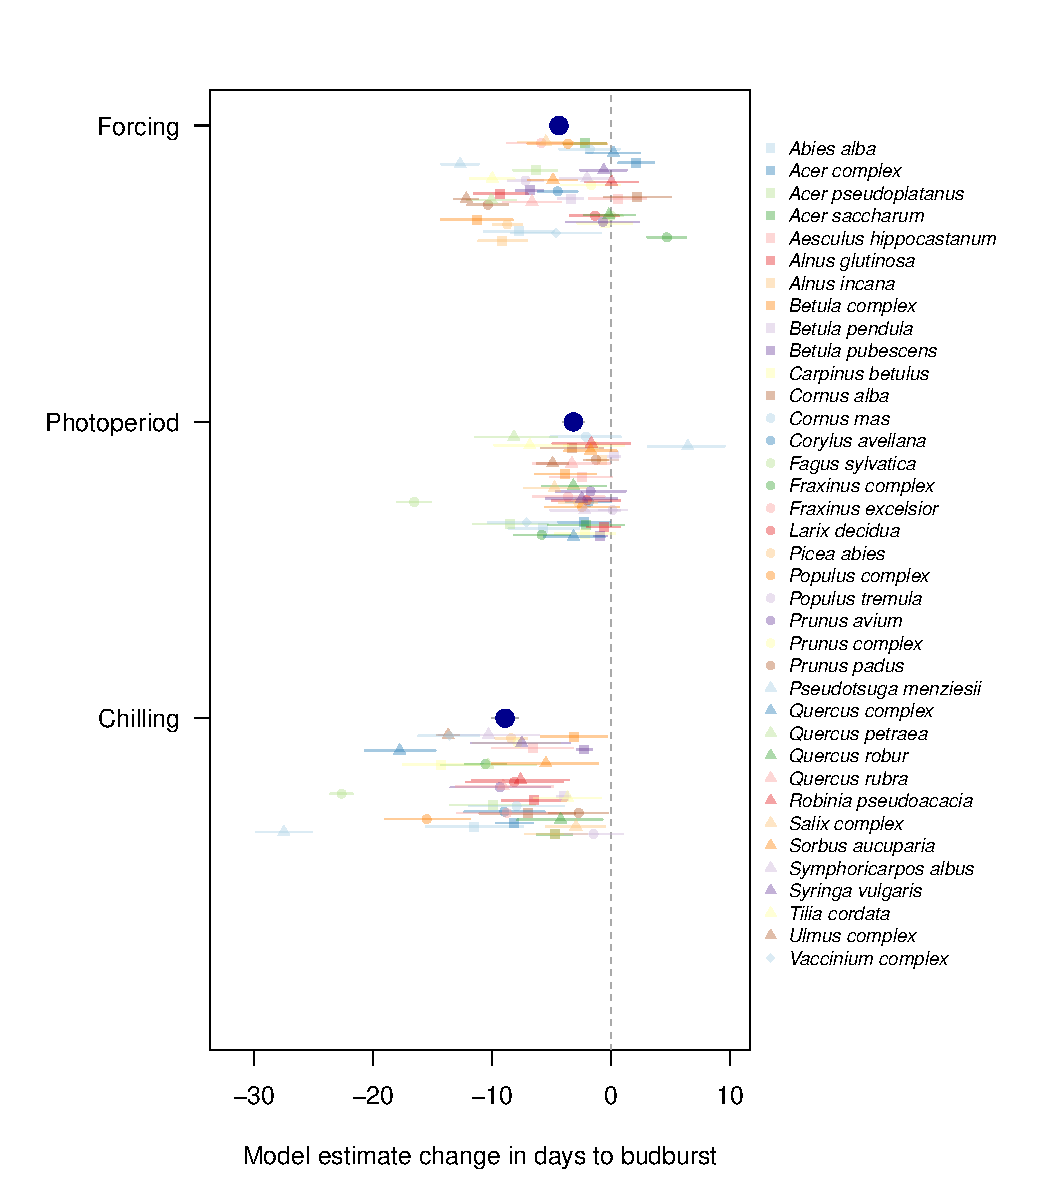
\includegraphics[width=0.75\textwidth]{..//..//analyses/bb_analysis/figures/muplotspcompexprampfputah_z.pdf}
\caption{\textbf{Estimated effects of chilling, forcing, and photoperiod on budburst timing across 42 controlled environment studies.} Using standardized units, which allow comparisons across cues, we show that most species (smaller symbols) are responsive to most cues, with chilling being the strongest cue when considering overall estimates across species (larger, dark blue circles). Overall estimates shown here were generally similar to other model formulations, including using data from 203 taxa, and using different methods for calculating chilling (Figs.\ref{fig:lat},\ref{fig:weinberger}; Tables \ref{tab:modsz}-\ref{tab:lat}). Lines represent 50\% uncertainty intervals (other intervals provided in Tables \ref{tab:modsz}-\ref{tab:lat})}.
\label{fig:mu}
\end{figure}

\newpage
%get min bb doy and associated chilling/forcing T

\begin{figure}[h!]
\centering
\noindent 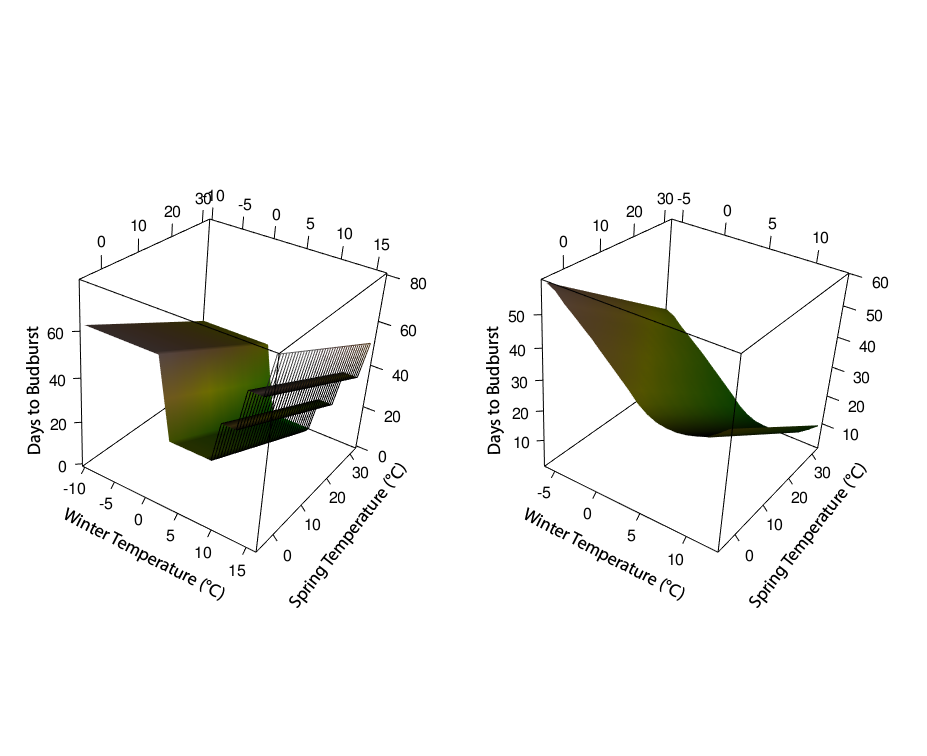
\includegraphics[width=0.75\textwidth]{..//..//analyses/bb_analysis/figures/bbmod_3dplot_utah_withPEP.png}
\caption{\textbf{Estimates of budburst across a range of forcing temperatures and estimated chilling} (converted to a representative mean temperature, see \emph{Estimating chilling} in the Supplemental Methods) based on overall estimates of chilling and forcing effects (Fig. 1). Maximum advances in budburst occur at intermediate chilling temperatures (e.g., here at 2818 chill units or a mean winter temperatures of 6.9 \degree C) and higher forcing (here at 8.8 \degree C). We set photoperiod to eight hours, which is the most common photoperiod treatment in the dataset. Note that days to budburst is relative to experimental methods and thus not comparable to day of year in the field, shading represents days to budburst.} % Adjust to maybe emphasize that it is a mix of the cues that determines when the earliest budburst happens *and* that these figures suggest at higher degrees of warming, when chilling declines, advances will slow or reverse.
\label{fig:apc}
\end{figure}
\newpage


\begin{figure}[h!]
\centering
\noindent 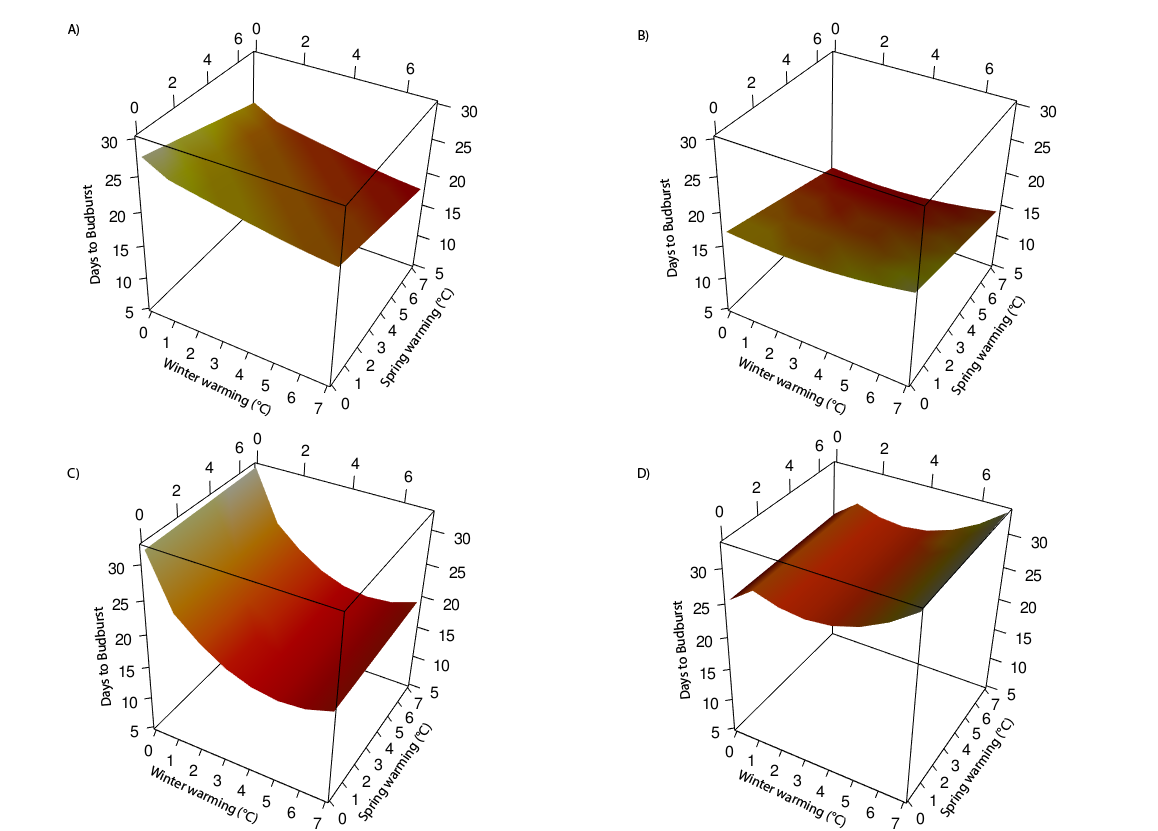
\includegraphics[width=0.75\textwidth]{..//..//analyses/bb_analysis/figures/forecasting/tempforecastbothspp_1_7_degwarm_3D_utah.png}
\caption{\textbf{Implications of warming on budburst timing varies across species and sites}, depending strongly on pre-warming climate conditions related to chilling for each site. Here we show species-level estimates from our model (Fig. \ref{fig:mu}) for the two most common species in the OSPREE database: \emph{Betula pendula} (A,B) and \emph{Fagus sylvatica} (C,D), for sites that highlight the diversity of possible budburst responses to warming (Fig. \ref{fig:foremap}, which shows general trends across many sites in Central Europe). In some sites, warming increases total chilling estimates (A, C) leading to greater advances in budburst (compared to forcing alone), whereas warming decreases total chilling estimates in other sites (B and D), leading to smaller advances, and eventually, delays with substantial warming. See Supplemental Materials, especially Fig. \ref{fig:foremap} - \ref{fig:chillfore}, for details.}
\label{fig:fore}
\end{figure}

%%%%%%%%%%%%%%%%%%%%%%%%%%%%%%%%%%%%%%%%
\end{document}
%%%%%%%%%%%%%%%%%%%%%%%%%%%%%%%%%%%%%%%%
